\chapter{Datasets Fisiológicos}


Apesar da existência de fontes de datasets fisiológicos públicos, 
o número de datasets disponíveis ainda é restrito. Sobre a qualidade das bases de dados, 
Mendoza et al. (2021) observou que nenhum de nove datasets disponíveis publicamente para 
treinamento de algoritmos de classificação analisados possuía 
todos os critérios de referência levantados por estudos anteriores, embora ainda mantivessem seu valor
para incentivar desenvolvimentos futuros.
Sobre a disponibilidade de datasets fisiológicos,
Rim et al. (2020) fez uma análise de datasets públicos e privados. 
No exemplo apresentado, 
é possível observar que datasets públicos combinando sinais são minoria nas diferentes fontes de dados analisadas
(figura 4.1).
s
\begin{figure}[!h]
      \centering
      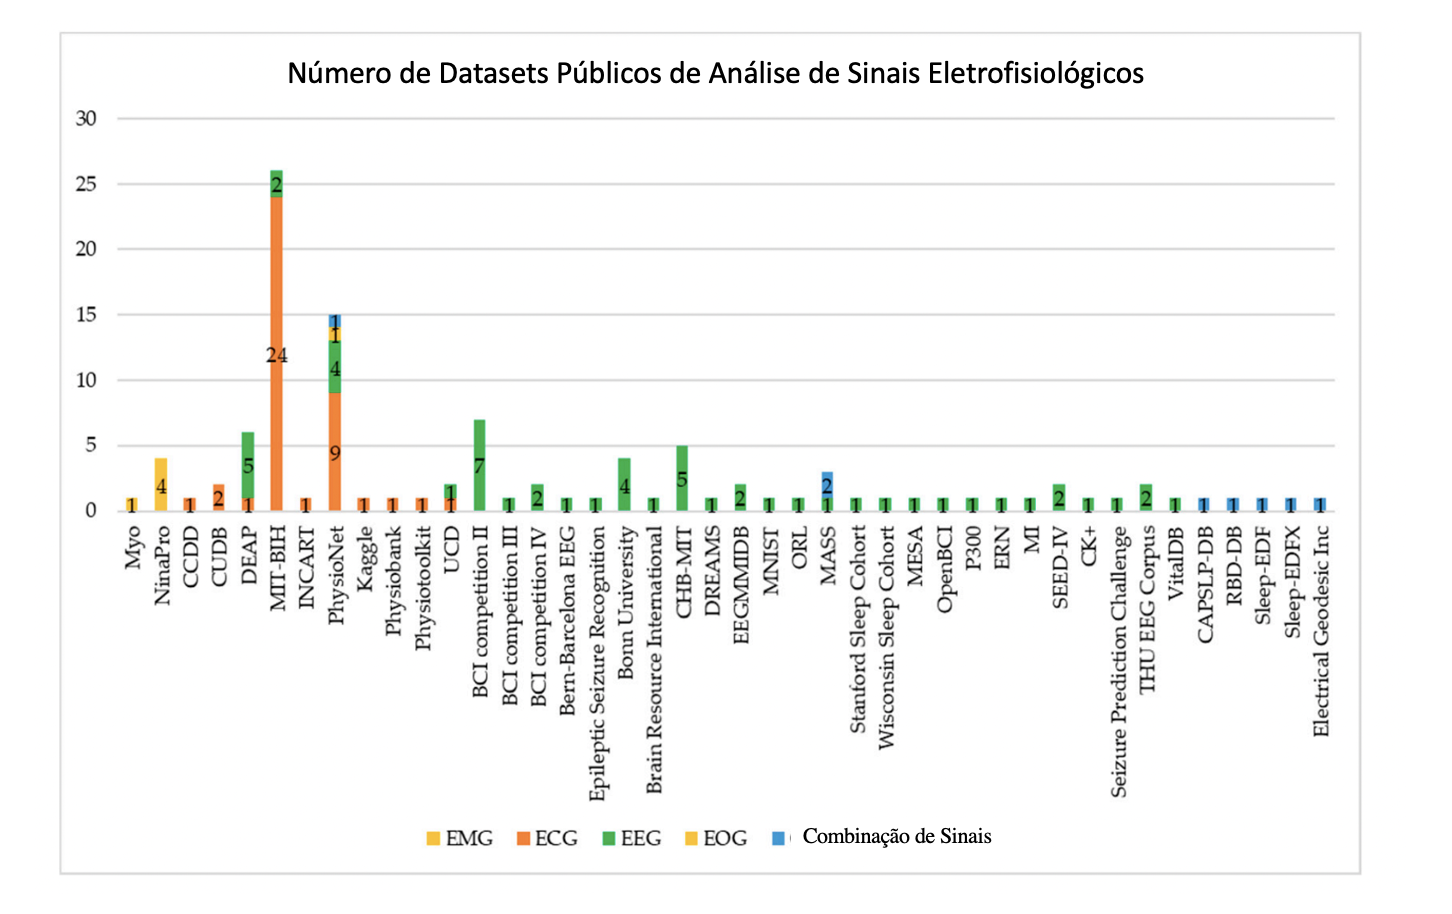
\includegraphics[width=160mm]{numero_datasets.png}
      \caption{Número de datasets disponíveis publicamente para estudos de sono por tipo de sinal. Fonte: Rim et al. (2020). }
\end{figure}

\section{Aquisição de EEG e ET}

Um exemplo de como se realizar a montagem para coleta de EEG e ET é demonstrado na figura 4.2, 
utilizado na montagem do dataset EEGEyeNet (Kastrati et al., 2021),
onde o participante é colocado de frente para o monitor para apresentação de estímulos com o 
equipamento de coleta de EEG sobre a cabeça e o aparelho de ET direcionado aos olhos. 


\begin{figure}[h]
      \centering
      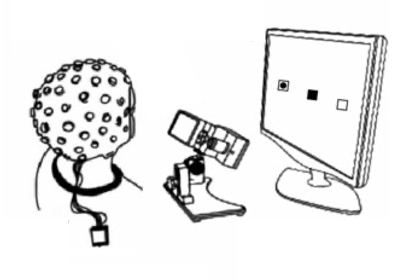
\includegraphics[width=80mm]{setup.png}
      \caption{Setup de coleta de EEG e ET. Fonte: Kastrati et al. (2021)}
\end{figure}



\section{Pré-processamento de EEG}
O pré-processamento de EEG consiste em remoção de artefatos, 
tais como contração muscular e movimentação ocular.
A etapa de extração de características consiste em, partindo dos dados com 
remoção de artefatos indesejáveis, extrair métricas estatísticas, como média, 
mediana e desvio padrão aplicados a uma janela de tempo, ou outras métricas, como entropia de Shannon 
(como feito no estudo de Thapaliya et al. (2019)). A seleção de features pode 
envolver o uso de algoritmos que permitem reduzir o número de características a 
serem apresentadas como input ao algoritmo, como o \textit{Principal Componen Analysis} (PCA).
 Um exemplo de pipeline é apresentado na figura 4.3. A partir dessas etapas, os dados são divididos entre treinamento e 
 teste, para validar o algoritmo ou algoritmos a serem estudados. 

 \begin{figure}[!h]
      \centering
      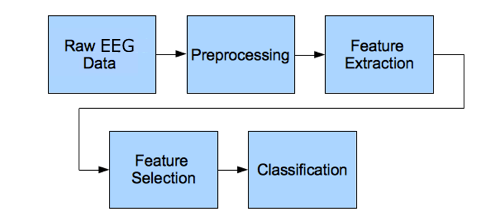
\includegraphics[width=100mm]{pipeline_eeg.png}
      \caption{Exemplo de pipeline para processamento de EEG. Fonte: Neuroeletrics (2022)}
 \end{figure}


 O pré-processamento será diferente dependendo se a fonte de dados é de \textit{single electrode} (somente um eletrodo)
 ou não, e do que é o sinal de interesse. Comumente não são estudados sinais acima de 90Hz (Neuroeletrics, 2022), 
 de forma que um filtro pode ser aplicado para remover frequencias que não forem de interesse. 
Também é comum dividir o sinal em épocas temporais de alguns segundos de duração, para extrair 
componentes destas janelas e construír a fase de extração de caractériscas. Esse processo acontece 
anteriormente a se inputar os dados a um modelo algoritmico. 

\section{A Fusão de Dados}
A fusão ou união de dados advindos de diferentes sensores pode ser realizada no nível de característica ou \textit{feature},
assim como a nível de decisão do algoritmo classificatório (Klein, 2014; Mendes et al., 2016).
      Na figura 4.4. é possível observar um fluxo de processamento dos sinais capturados por diferentes sensores.  Os diferentes 
      sensores representados no estudo de Mendes et al. (2016) são aqui representados pela coleta de EEG e ET.
 
\begin{figure}
      \centering
      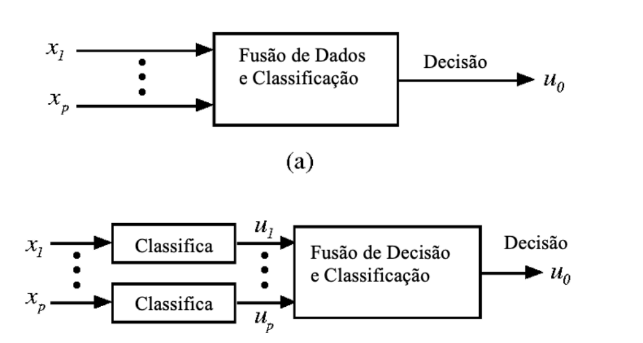
\includegraphics[width=100mm]{fusao_decisao.png}
      \caption{Exemplo de Fluxo para Fusão de Dados de Sensores. Fonte:  Mendes et al. (2016)}
\end{figure}


Na \textit{\textbf{Feature Level Fusion}} (FLF), os dados de diversas fontes são extraídos dos sensores e unidos de forma a 
gerar um vetor único com informações multimodais; no \textit{\textbf{Decision Fusion}} (DL) a classificação ocorre para cada categoria 
de fonte de dado (exemplo: uma classificação para EEG e outra para ET) e estas 
classificações são combinadas em um esquema de voto (exemplo: a classificação mais comum) 
para se chegar em uma categoria final (Bota et al., 2020). A respeito de qual formato seria melhor, 
Bota et al. (2020) observou que o melhor método de fusão é altamente correlacionado à base dados, 
embora o FLF tenha sido escolhido como o melhor em função de sua baixa complexidade em relação ao DF. 




